%!TEX root = ../main.tex
\section{Board Design} % (fold)
\label{sec:board_design}
Multiple electronics components are required to realise the double pendulum being developed throughout this report.
This section explores the design of those components and the communication between them.
Most of the circuitry is combined on a single PCB, the driver board, however some of the functionality is moved to smaller boards, local to the place where they are needed.\\

The components of the system are listed here:
\begin{itemize}
	\item Motor Encoder
	\item Joint Encoder
	\item End Stops
	\item Motor Driver
	\item Emergency Circuitry
	\item Relay Driver
	\item RF Transceiver
	\item MicroZed 
\end{itemize}
Many of these components require a number of subcomponents, which will be explored further in later sections.

\subsection{Voltage Rails} % (fold)
\label{sub:voltage_rails}
In the design of the board it is necessary to determine which voltage rails are required for the system to function.
The power delivery for the MicroZed was designed by the authors in an earlier project \cite{isaswarm} and will be reused with minor changes.
This power delivery system provides, amongst other voltages, the 3.3V rail, originally intended for powering the MicroZed IO banks only.
In this system however, the RF tranceiver is also powered from this rail.
As a result a review of the circuitry around the 3.3V rail is necessary to ensure that it can provide the required power.
The MicroZed power delivery system, the encoders of the system, the endstops and part of the emergency circuitry are all driven from a 5V rail.
The Motor Driver, the HIP4081 \cite{driver} and the relay driving circuitry is driven from a 12V rail.
Finally, the motor is driven from a 24V rail, which will also be the main supply for the system.
This rail is not crucial to the design of the board as it is provided by an external, mains connected power supply and will not be explored further in this section.\\
The current requirement for each of these rails are discussed in the following paragraphs

\paragraph{3.3V:} % (fold)
\label{par:3_3v}
As mentioned, this rail is intended for powering the MicroZed IO banks.
In the original design the LMR10510XMF DC/DC converter is used to provide the necessary power.
This chip is capable of supplying up to 1A.
Components exist in the same series which are pin compatible and are capable of supplying up to 2A.
The RF Transceiver used in this project, however, \ref{} requires only up to 15mA when receiving data.
Assuming that Avnet has already provided headroom for the IO bank supply and considering that this project makes little use of the IO on the Zynq-7000 chip, it is deemed unnecessary to upgrade this supply and the original design is used as is.
% paragraph 3_3v_ (end)

\paragraph{5V:} % (fold)
\label{par:5v}
This rail supplies, mainly, the MicroZed.
The authors previously found \cite{isaswarm} that the maximum expected current draw seen from the MicroZed is 1.85A at 5V.
In addition, in this design, the 5V rail also powers the encoders, endstops and emergency circuitry.
There are two types of encoders, the HEDS-5540 \cite{heds5540}, which requires a maximum of 85mA and a Rolin magnetic encoder, which requires a maximum of 25mA.\\
The endstops are realised using the TCST2103 infrared sensor \cite{tcst2103}.
The majority of the current supplied to this sensor is used to power the infrared LED present in the component.
This current is decided by the resistor put in series with the LED and is estimated to be around 50mA per LED for a total of 100mA.
Another 10mA is added to that figure due to the collector current possible on the transistor side.\\
Finally the emergency circuitry along with some other digital electronics are powered from the 5V rail.
As these are all digital IC's that operate on nothing but signals, their individual powers are negligible but a very conservative 25mA power budget is provided for all of the digital electronics on the 5V rail. This brings the total power budget for the 5V rail to $\approx$2.1A.
See table \ref{tab:5vpowerbudget} for a full overview.

\begin{table}
	\centering
	\begin{tabular}{l|r}
		 Component & Current [mA]\\
		 \hline
		 MicroZed & 1850\\
		 HEDS-5540 & 85\\
		 Rolin Enc. & 25\\
		 TCST2103 & 110\\
		 Digital & 25\\
		 \hline
		 Total & 2095
	\end{tabular}
	\caption{Power budget for the 5V rail}
	\label{tab:5vpowerbudget}
\end{table}

In \cite{isaswarm} the authors used a design in which the PTH08080 is used to generate a 5V rail.
Reusing this module will save on design time as well as the budget available to the project and as such is desirable.
This module however, is capable of supplying only 2A at 5V, slightly less than the value calculated in this section.
By far the largest contributor to the power budget is the MicroZed.
The calculation of the contribution from the MicroZed is done assuming 85\% utilisation of PL and a conservative 80\% efficiency of internal DC/DC converters.
Considering this, it is safe to assume that the real power draw from the MicroZed is significantly smaller than the calculated value and as a result it is chosen to reuse the PTH08080 despite of apparent shortcomings of the module.
% paragraph 5 (end)

\paragraph{12V:} % (fold)
\label{par:12v}
This rail powers the HIP4081 motor driver, the relay coils, the bootstrap circuitry and the 5V DC/DC converter.
The PTH08080 DC/DC converter has a maximum input voltage of 18V and must be powered from the 12V rail rather than the 24V rail.
The module can provide 2A at 5V and as such will require $\approx$0.85A from the 12V rail.\\
There are two relays in the design, a smaller relay for controlling the inrush current and the larger main supply relay.
Both of these require power to stay in the closed position.
The first, the G6B \cite{g6b}, requires 16.7mA while the former, the LEV100A4ANG \cite{lev100}, requires 461mA.\\
The motor driver of the system, the HIP4081 requires only 10mA.
As mentioned, the bootstrap circuitry is also powered from the 12V rail.
Rather than a steady supply, this circuitry requires a large peak current for short periods while charging in between switching.
For this reason the design choice here is to determine what is available and choose the component which yields the most headroom while still being economically feasible.
Amongst all of the components the total power budget for the 12V rail is $\approx$1340mA.
See table \ref{tab:12vpowerbudget} for a full overview.

\begin{table}
	\centering
	\begin{tabular}{l|r}
		 Component & Current [mA]\\
		 \hline
		 PTH08080 & 850\\
		 G6B & 16.7\\
		 LEV100A4ANG & 461\\
		 HIP4081 & 10\\
		 \hline
		 Total & 1337.7
	\end{tabular}
	\caption{Power budget for the 12V rail}
	\label{tab:12vpowerbudget}
\end{table}

The PTN78020 delivers 6A at 12V and is part of the same series as the PTH08080 described earlier.
This allows many of the same design procedures to be reused.
In addition, the 6A current limit leaves sufficient room for the current spikes expected from the bootstrap circuitry.
The bootstrap circuitry is modified slightly to accomodate the limited supply as described in section \ref{}
% paragraph 12v_ (end)

% subsection voltage_rails (end)

% section board_design (end)


\subsection{PTN78020H Circuit}
\mikkel{A wild subsection appears! (Should be moved to a section where it makes sense)}
\begin{figure}
	\centering
	\includegraphics[width=\linewidth]{graphics/}
	\caption{Caption here}
	\label{fig:figure1}
\end{figure}
The \texttt{PTN78020H} DC/DC converter is used to generate the 12V rail. 
The component requires input and output capacitors in order to function properly and a resistor is needed to set the wanted output voltage. 
According to the components datasheet \cite{PTN78020H}, a 1\% 383 k$\Omega$ is needed to generate an output voltage of 12V.
The datasheet furthermore specifies that ceramic capacitance of 18.8 $\mu$F is needed at the input. 
It was chosen to use two 0805 10 $\mu$F capacitors.
In order to ensure stability the \texttt{PTN78020H} needs an output capacitance of 330 $\mu$F.
The datasheet specifies that if the application has load transients additional capacitance should be added to improve the response of the regulator. 
It was therefore decided to add two 330 $\mu$F in parallel. 
Two 10 $\mu$F ceramic capacitors are placed at the output to further improve the transient response. 
\mikkel{Figure?}



\subsection{Current Measuring}
\mikkel{A wild subsection appears! (Should be moved to a section where it makes sense)}
While reading in the literature it was found that measuring the current through the motor is beneficial for controlling the pendulums.

Current measurements are generally done by either hall effect based sensors or shunt resistors. 
Hall effect based sensors are generally the expensive solution and measuring small currents can be problematic. 
Therefore it was chosen to use a shunt resistor.
The basic idea is to place a resistor with a very low resistance in series with the load which current should be measured. 
Measuring the motor current when using a H-bridge can be done in a various of ways.
The three main ones are high-side, in-line and low-side placement of the shunt resistor as shown in figure \ref{fig:shunt_measure_high_in_low}.

\begin{figure}[h]
	\centering
    %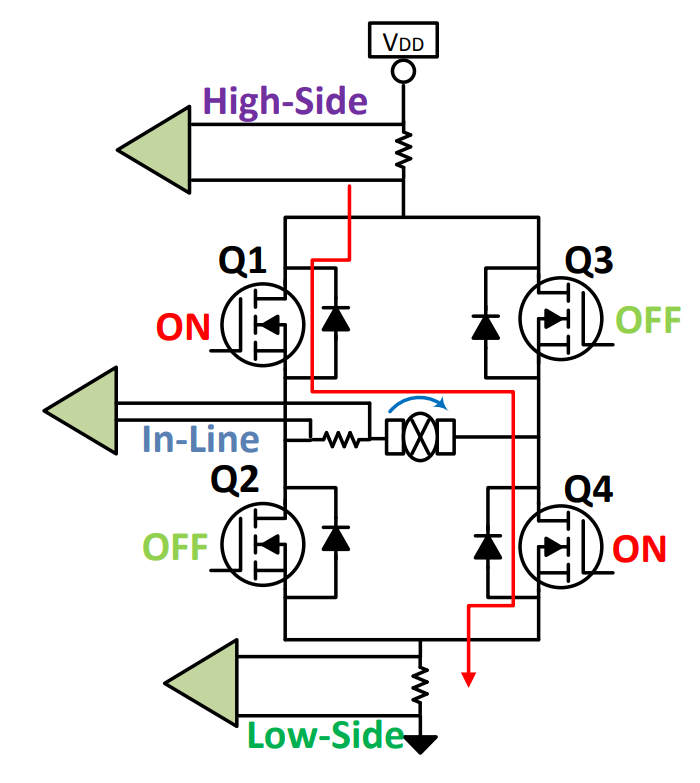
\includegraphics[width=0.5\linewidth]{graphics/shunt_sense_high_in_low}
	\caption{xxxx.}
	\label{fig:shunt_measure_high_in_low}
\end{figure}
\mikkel{Figure should be replaced by own illustration}

\cite{shunt_placement} and \cite{Current_Sense_Circuit_Collection} specifies the advantages and disadvantages of the three configurations. 
Based on that it was decided to use the low-side configuration as it has low common voltage, it only needs a single sided supply and bi-directional current measurement is not needed.


\subsubsection{Requirements for the Current Measuring Circuit}
The output of the current measuring circuit is an analogue signal that needs to be measured by the ADC of the Zynq chip.
According to the Zynqs ADC user guide \cite{zynq_adc}, the measurable input range is from 0V to 1V, but the maximum allowed input voltage is 1.9V according to \cite{adc_zynq_webanswer}.
The absolute maximum current through the motor is the stall current which is 80A, but the motor will run at well below this level in normal operation.
The normal operation currents are expected to be up to 30A???(needs explanation somewhere...).
It was therefore decided that the circuit  needs to be able to measure currents of at least up to 40A.
The resolution per Ampere is increased by decreasing the current range that can be measured,
If the current gets any higher the ADC input should not be harmed meaning that the input voltage should not exceed 1.9V.

\mikkel{Below should be formatted differently}
\textbf{Requirements for the circuit:}
\begin{itemize}
	\item ADC input voltage does not exceed 1.9V when motor is stalling.
	\item Measures currents up to 40A, at minimum.
\end{itemize}


\subsubsection{Designing the Current Measuring Circuit}
The requirements listed above can be realized in a number of ways by choosing resistance of the shunt resistor and gain of the current-sense amplifier.
It was chosen to use a 200 $\mu \Omega$ SMD shunt resistor, as it is was the smallest resistance available at the university's electronics supplier. 
Such a small resistance yields a minimal voltage drop and thus a minimal power consumption.
The \texttt{INA286AID} from Texas Instruments was chosen as the current-sense amplifier, because is has all the wanted features, has a gain of 100 and a very low offset allowing it to be used in applications where the maximum voltage drop across the shunt resistor is 10 mV full-scale \cite{INA286AID}.
Using these components the stalling current of 80A will result in input voltage to the ADC of 1.6 V as shown in \ref{eq:adc_input_voltage1} and \ref{eq:adc_input_voltage2}.

\begin{equation}
	V_{max,input} = G \cdot V_{shunt}
	\label{eq:adc_input_voltage1}
\end{equation}
\begin{equation}
	V_{max,input} = G \cdot R_{shunt} \cdot I_{stall} = 100 \cdot 200\cdot10^{-6} \cdot 80 = 1.6V
	\label{eq:adc_input_voltage2}
\end{equation}

The maximum current that can be measured is 50A as shown in \ref{eq:adc_input_voltage3}.

\begin{equation}
	I_{max, measurable} = \frac{V_{max, measurable}}{R_{shunt}\cdot G} = \frac{1}{100 \cdot 200\cdot10^{-6} } = 50A
	\label{eq:adc_input_voltage3}
\end{equation}

These results clearly shows that the design meets the requirements.
